% !TEX program = lualatex
\documentclass[aspectratio=43,professionalfonts,handout]{beamer}
\usepackage{beamer_template}

\newcommand{\LectureNum}{13}
\newcommand{\LectureTitle}{逆関数}
\newcommand{\TextPages}{p.\,96-97}
\newcommand{\NextTopic}{問題演習}
\newcommand{\NextPages}{p.\,98-100（練習問題2-A, 2-B）}
\newcommand{\CourseName}{基礎数学B}
\renewcommand{\TermName}{前期}

\begin{document}

% -----------------------------------------------
% スライド1: 表紙＋目標＋用語・定義
% -----------------------------------------------
\begin{frame}{\CourseName\quad 第\LectureNum 回「\LectureTitle 」}
  {\small \TermName\quad \TeacherName\quad ／\quad 教科書 \TextPages\quad
  \textbf{目標}：逆関数の定義と求め方を理解し、y=x に関する対称性を説明できる}

  \begin{block}{用語・定義}
  \begin{description}[labelwidth=5.5em]
    \item[\kw{逆関数}] ~
    \item[\kw{定義域と値域の入れ替わり}] ~
    \item[\kw{y=x に関する対称性}] ~
  \end{description}
  \end{block}
\end{frame}

% -----------------------------------------------
% スライド2: 公式・性質
% -----------------------------------------------
\begin{frame}{公式・性質}
  \begin{block}{}
  \begin{itemize}
    \item 逆関数の求め方3ステップ
    \item 逆関数が存在する条件（1対1）
    \item 例：y=x²（x≧0）→ y=√x
  \end{itemize}
  \end{block}
\end{frame}

% -----------------------------------------------
% スライド3: 図・グラフ（TikZコードを手動追加）
% -----------------------------------------------
\begin{frame}{図・グラフ}
  \centering
  % TODO: y=x²-1（x≧0）と逆関数 y=√(x+1)、y=x に関する対称性
  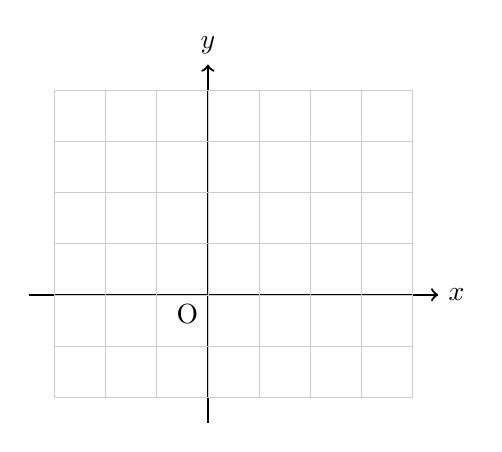
\begin{tikzpicture}[scale=0.65]
    \draw[->,thick] (-3.5,0) -- (4.5,0) node[right]{$x$};
    \draw[->,thick] (0,-2.5) -- (0,4.5) node[above]{$y$};
    \node[below left] at (0,0) {O};
    \draw[gray!40, very thin] (-3,-2) grid (4,4);
    % ここにグラフを描画
  \end{tikzpicture}
\end{frame}

% -----------------------------------------------
% スライド4: 例1→問1
% -----------------------------------------------
\begin{frame}{例1→問1}
  \begin{exampleblock}{例題3) p.96（逆関数を求める）}
    （板書で解説）
  \end{exampleblock}

  \vfill

  \begin{block}{問9) p.97（3問）\quad 自分で解いてみよう}
    （ノートに解くこと）
  \end{block}
\end{frame}

% -----------------------------------------------
% スライド5: 例2→問2
% -----------------------------------------------
\begin{frame}{例2→問2}
  \begin{exampleblock}{練習2-A 問6) p.99（逆関数とグラフ）}
    （板書で解説）
  \end{exampleblock}

  \vfill

  \begin{block}{練習2-A 問7) p.99\quad 自分で解いてみよう}
    （ノートに解くこと）
  \end{block}
\end{frame}

% -----------------------------------------------
% まとめ
% -----------------------------------------------
\begin{frame}{まとめ}
  \begin{itemize}
    \item 逆関数は x と y を入れ替えて y について解く
    \item もとの関数の定義域・値域と逆関数の値域・定義域は入れ替わる
    \item y=f(x) と逆関数のグラフは直線 y=x に関して対称
  \end{itemize}

  \vfill
  {\small 基本問題：179}
\end{frame}

\end{document}
